%!TEX program = xelatex

% \documentclass[10pt]{article}
%%%%%%%%%%%%%%%%%%%%%%%%%%%%%%%%%%%%%%%%%
% Modified By Orcuslc, 2016-9-12
% http://github.com/orcuslc
%
% Wilson Resume/CV
% Structure Specification File
% Version 1.0 (22/1/2015)
%
% This file has been downloaded from:
% http://www.LaTeXTemplates.com
%
% License:
% CC BY-NC-SA 3.0 (http://creativecommons.org/licenses/by-nc-sa/3.0/)
%
%%%%%%%%%%%%%%%%%%%%%%%%%%%%%%%%%%%%%%%%%

%----------------------------------------------------------------------------------------
%	PACKAGES AND OTHER DOCUMENT CONFIGURATIONS
%----------------------------------------------------------------------------------------

\usepackage[a4paper, hmargin=25mm, vmargin=30mm, top=20mm]{geometry} % Use A4 paper and set margins

\usepackage{fancyhdr} % Customize the header and footer

\usepackage{lastpage} % Required for calculating the number of pages in the document

\usepackage{hyperref} % Colors for links, text and headings

\setcounter{secnumdepth}{0} % Suppress section numbering

%\usepackage[proportional,scaled=1.064]{erewhon} % Use the Erewhon font
%\usepackage[erewhon,vvarbb,bigdelims]{newtxmath} % Use the Erewhon font
\usepackage[utf8]{inputenc} % Required for inputting international characters
\usepackage[T1]{fontenc} % Output font encoding for international characters

\usepackage{fontspec} % Required for specification of custom fonts
\setmainfont[Path = ./fonts/,
Extension = .otf,
BoldFont = Erewhon-Bold,
ItalicFont = Erewhon-Italic,
BoldItalicFont = Erewhon-BoldItalic,
SmallCapsFeatures = {Letters = SmallCaps}
]{Erewhon-Regular}

\usepackage{color} % Required for custom colors
\definecolor{slateblue}{rgb}{0.17,0.22,0.34}

\usepackage{sectsty} % Allows customization of titles
\sectionfont{\color{slateblue}} % Color section titles

\fancypagestyle{plain}{\fancyhf{}\cfoot{\thepage\ of \pageref{LastPage}}} % Define a custom page style
\pagestyle{plain} % Use the custom page style through the document
\renewcommand{\headrulewidth}{0pt} % Disable the default header rule
\renewcommand{\footrulewidth}{0pt} % Disable the default footer rule

\setlength\parindent{0pt} % Stop paragraph indentation

% Non-indenting itemize
\newenvironment{itemize-noindent}
{\setlength{\leftmargini}{0em}\begin{itemize}}
{\end{itemize}}

% Text width for tabbing environments
\newlength{\smallertextwidth}
\setlength{\smallertextwidth}{\textwidth}
\addtolength{\smallertextwidth}{-2cm}

\newcommand{\sqbullet}{~\vrule height 1ex width .8ex depth -.2ex} % Custom square bullet point definition

%----------------------------------------------------------------------------------------
%	MAIN HEADER COMMAND
%----------------------------------------------------------------------------------------

\renewcommand{\title}[1]{
{\huge{\color{slateblue}\textbf{#1}}}\\ % Header section name and color
\rule{\textwidth}{0.5mm}\\ % Rule under the header
}

%----------------------------------------------------------------------------------------
%	JOB COMMAND: Modified by Orcuslc 2016-09-12
%----------------------------------------------------------------------------------------

\newcommand{\job}[6]{
\begin{tabbing}
\hspace{2cm} \= \kill
\textbf{#1} \> \href{#4}{\textbf{#3}} \\
\textbf{#2} \>\+ \textit{#5} \\
\begin{minipage}{\smallertextwidth}
\vspace{2mm}
#6
\end{minipage}
\end{tabbing}
\vspace{2mm}
}

%----------------------------------------------------------------------------------------
%	SKILL GROUP COMMAND - Modified by Orcuslc 2016-09-12
%----------------------------------------------------------------------------------------

\newcommand{\skillgroup}[2]{
% \begin{tabbing}
% \hspace{5mm} \= \kill
% \sqbullet \> \textbf{#1}
% \end{tabbing}
% \begin{tabbing}
% \vspace{-2pt}
% \hspace{3cm} \= \kill
% #2
% \end{tabbing}
% }
\begin{tabbing}
\hspace{5mm} \= \kill
\sqbullet \>\+ \textbf{#1} \\

\begin{minipage}{\smallertextwidth}
\vspace{2mm}
#2
\end{minipage}
\end{tabbing}
}

\newcommand{\skill}[2]{
\begin{tabbing}
\hspace{1cm} \> \hspace{3cm} \= \kill
\>\textbf{#1:} \> #2 \\
\end{tabbing}
% \hspace
}

%----------------------------------------------------------------------------------------
%	INTERESTS GROUP COMMAND
%-----------------------------------------------------------------------------------------

\newcommand{\interestsgroup}[1]{
\begin{tabbing}
\hspace{5mm} \= \kill
#1
\end{tabbing}
\vspace{-10mm}
}

\newcommand{\interest}[1]{\sqbullet \> \textbf{#1}\\[3pt]} % Define a custom command for individual interests


%---------------------------------------------------------------
%   AWARDS GROUP COMMAND: Created by Orcuslc 2016-09-12
%---------------------------------------------------------------
\newcommand{\awardgroup}[1]{
\begin{tabbing}
\hspace{5mm} \= \kill
#1
\end{tabbing}
\vspace{2mm}
}

\newcommand{\award}[2]{
% \begin{tabbing}
% \hspace{0} \> \hspace{2cm} \= \kill
\hspace{2cm} \> \hspace{2cm} \= \kill
\sqbullet \> \textbf{#1} \> #2 \\[3pt]
% \hspace{2cm} \= \kill
% \end{tabbing}

}

%----------------------------------------------------------------------------------------
%	TABBED BLOCK COMMAND: Modified by Orcuslc 2016-09-12
%----------------------------------------------------------------------------------------

\newcommand{\tabbedblock}[1]{
\begin{tabbing}
\hspace{2cm} \= \hspace{4cm} \= \hspace{4cm} \= \hspace{4cm} \= \kill
#1
\end{tabbing}
}

%-----------------------------------------------------------------
%  TABBED BLOCK 2 COMMAND: Created by Orcuslc 2016-09-12
%-----------------------------------------------------------------
\newcommand{\tabblock}[5]{
\begin{tabbing}
% \hspace{2cm} \= \kill
\hspace{2cm} \= \hspace{4cm} \= \hspace{4cm} \= \hspace{4cm} \= \kill

\textbf{#1} \> \textbf{#3} \\
\textbf{#2} \> \textbf{#4} \\[5pt]
\>\+
#5
\end{tabbing}
}


%-----------------------------------------------------------------
%  RESEARCH COMMAND: Created by Orcuslc 2016-09-12
%-----------------------------------------------------------------
\newcommand{\research}[7]{
\begin{tabbing}
\hspace{2cm} \= \kill
\textbf{#1} \> \textbf{#3}, under the supervision of \href{#5}{\textbf{#4}} \\
% \href{#4}{#3} \\
\textbf{#2} \>\+ \textit{#6} \\
\begin{minipage}{\smallertextwidth}
\vspace{0.5mm}
#7
\end{minipage}
\end{tabbing}
\vspace{2mm}
}

%-------------------------------------------------------------------------
%      Programming Projects Command - Created by Orcuslc 2016-9-14
%-------------------------------------------------------------------------
% \newcommand{\projectgroup}[1]{
% \begin{tabbing}
% % \hspace{5mm} \= \kill
% \vspace{5mm}
% #1
% \end{tabbing}
% }

\newcommand{\projectgroup}[1]{
% \begin{tabbing}
\hspace{5mm} \= \kill
#1
% \end{tabbing}
\vspace{2mm}
}


\newcommand{\project}[3]{
% \begin{tabbing}
\hspace{2cm} \> \hspace{2cm} \= \kill
\sqbullet \> \textbf{#1} \> #2 \\
\> \textbf{code:} \> \href{#3}{#3} \\[5pt]
% \end{tabbing}
}
\usepackage{epstopdf}
\usepackage{graphics}
\usepackage{subfig}
\usepackage{float}
\usepackage{listings}
\lstset{
  numbers=left,
    framexleftmargin=10mm,
    frame=none,
    backgroundcolor=\color[RGB]{245,245,244},
  keywordstyle=\bf\color{blue},
  identifierstyle=\bf,
  numberstyle=\color[RGB]{0,192,192},
  commentstyle=\it\color[RGB]{0,96,96},
  stringstyle=\rmfamily\slshape\color[RGB]{128,0,0},
  showstringspaces=false,
  extendedchars=false
    }
\DeclareGraphicsExtensions{.eps,.ps,.jpg,.bmp}

\begin{document}

\title{Homework 3}{16.11.4}

% \parbox{0.3\textwidth}{
% Chuan Lu}
% \hfill
% \parbox{0.3\textwidth}{
% 13300180056}
% \hfill
% \parbox{0.3\textwidth}{
% chuanlu13@fudan.edu.cn}

\problem{1}{Perform PCA to assign31.csv.}
\solution{Result}{
Since there are many NAs in assign31.csv, I changed those NA to 0. \n
The results are as follows: The rate in the table is the rate of information reserved after PCA.
\begin{table}[htbp] \large \centering
\begin{tabular}{|c|c|c|c|c|c|c|}
\hline
k & 1 & 2 & 3 & 5 & 10 & 14  \\
\hline
Rate & 0.2139058 &  0.396026 & 0.5165856 & 0.6697862 & 0.920202 & 1\\
\hline
\end{tabular}
\caption{Reserved information rate of different orders in PCA.}
\end{table}
\begin{figure}[H]
\centering
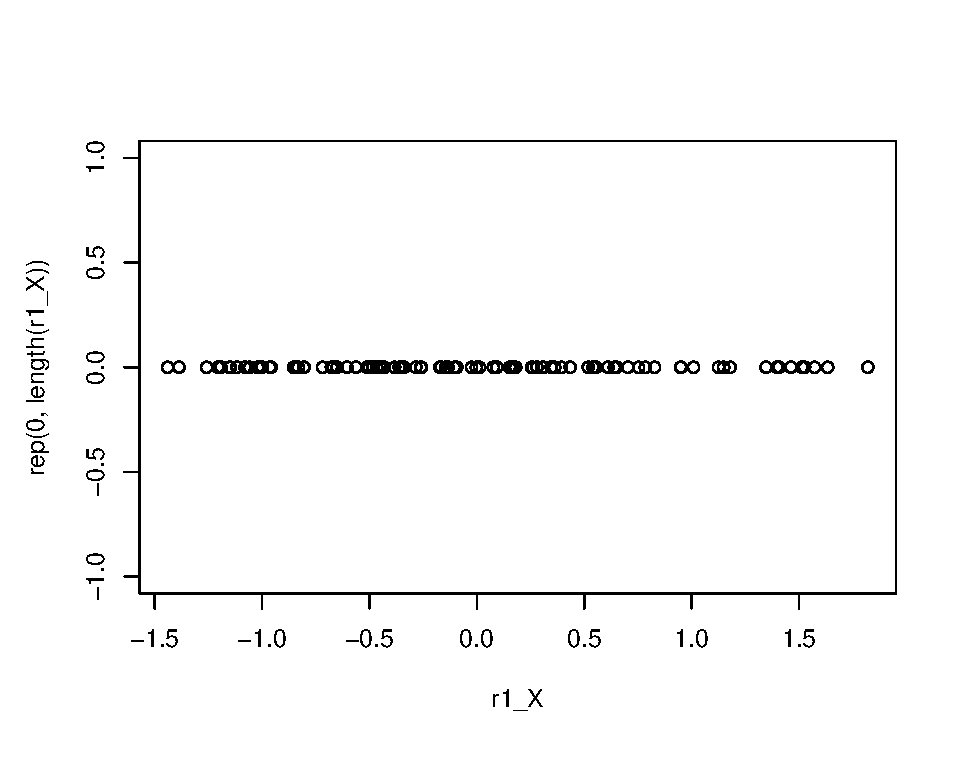
\includegraphics[width = 15cm]{pics/hw1_pca_1.eps}
\caption{PCA, k = 1}
\label{PCA1}
\end{figure}
\begin{figure}[H]
\centering
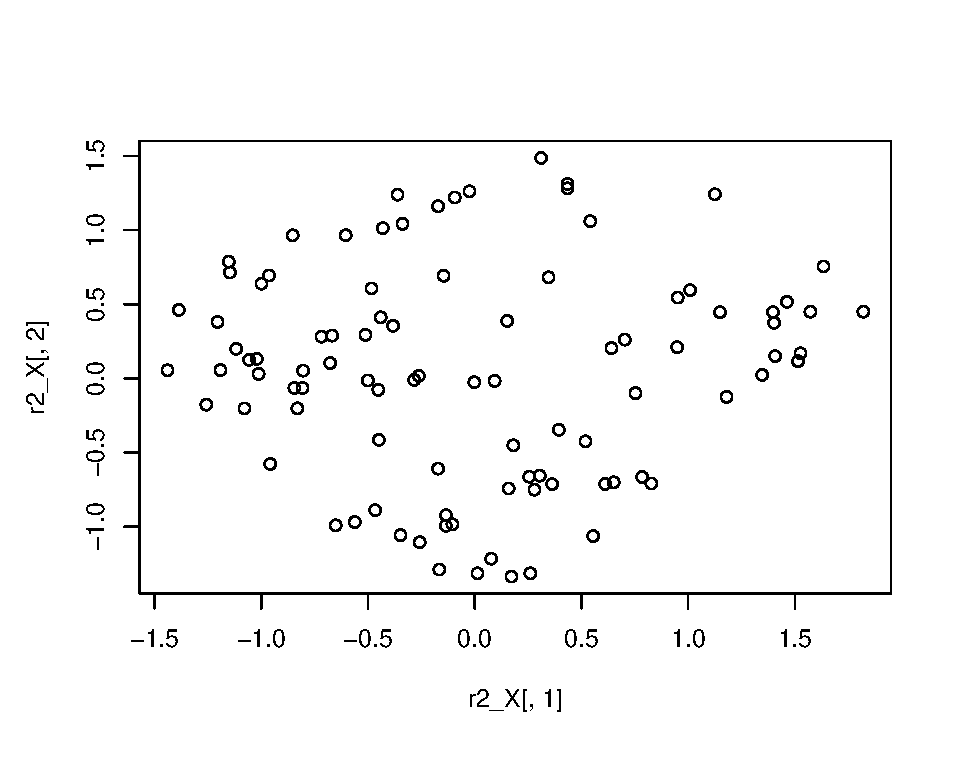
\includegraphics[width = 15cm]{pics/hw1_pca_2.eps}
\caption{PCA, k = 2}
\label{PCA2}
\end{figure}
\begin{figure}[H]
\centering
\includegraphics[width = 15cm]{pics/hw1_pca_3.png}
\caption{PCA, k = 3}
\label{PCA3}
\end{figure}
From these figures(when $k = 1, 2, 3$) we can find that after PCA the data points still seem to be random and messy. When we calculate the rate of reserved information we can know that not until $k = 10$ the rate is less than 0.9, which is thought to be unsatisfying.
}


\problem{2}{Perform PCA and NMF to assign2.csv, and explain the difference.}
\solution{Result}{
For PCA, the result is as follows:
\begin{table}[htbp] \large \centering
\begin{tabular}{|c|c|c|c|}
\hline
k & 1 & 2 & 3  \\
\hline
Rate & 0.4326317 &  0.7648243 & 0.9298461 \\
\hline
\end{tabular}
\caption{Reserved information rate of different orders in PCA.}
\end{table}
\begin{figure}[H]
\centering
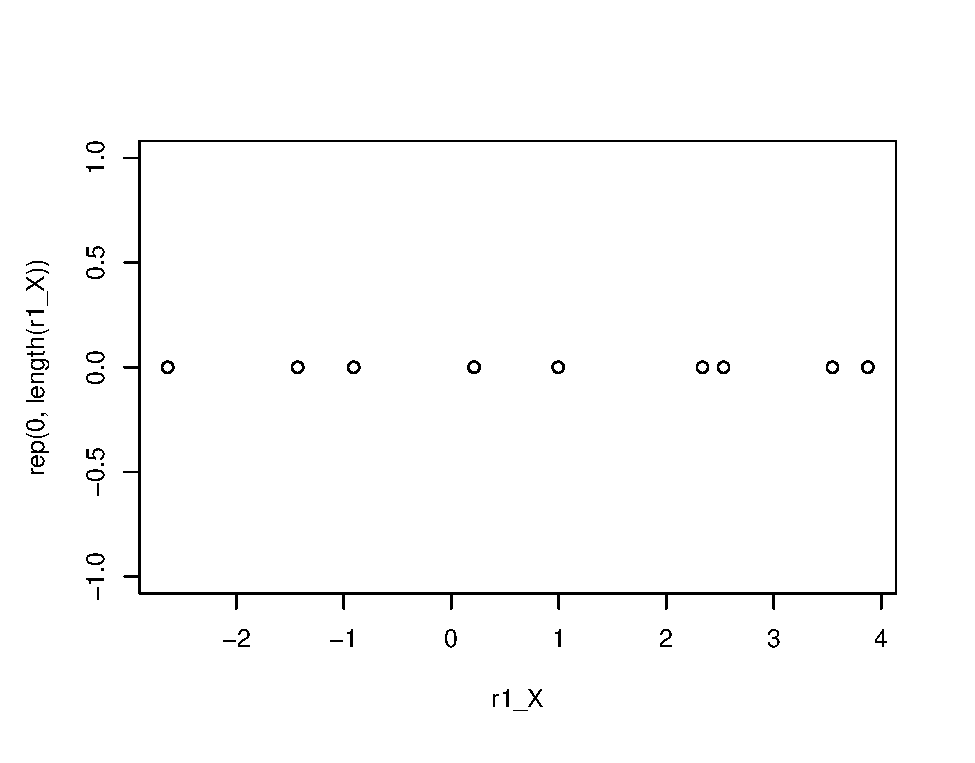
\includegraphics[width = 15cm]{pics/hw2_pca_1.eps}
\caption{PCA, k = 1}
\label{PCA2_1}
\end{figure}
\begin{figure}[H]
\centering
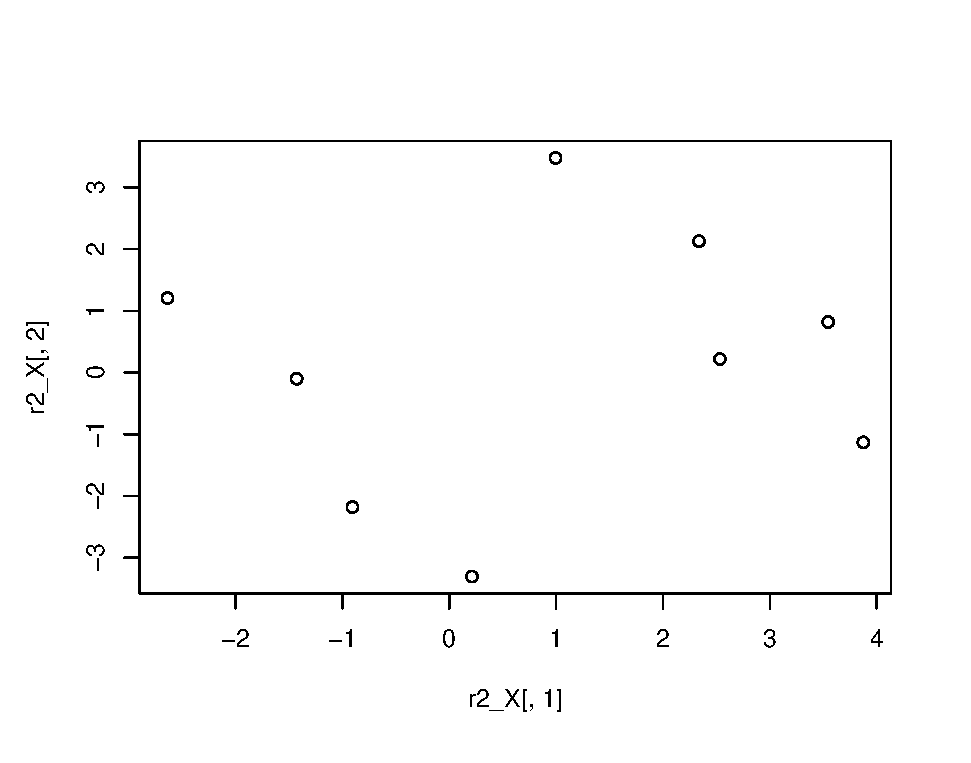
\includegraphics[width = 15cm]{pics/hw2_pca_2.eps}
\caption{PCA, k = 2}
\label{PCA2_2}
\end{figure}
\begin{figure}[H]
\centering
\includegraphics[width = 15cm]{pics/hw2_pca_3.png}
\caption{PCA, k = 3}
\label{PCA2_3}
\end{figure}
From figure(k = 1) we can assert nothing; from figure(k = 2) it seems the data can be simulated by two parallel lines. From the table we can find when k = 3, the rate of reserved information is over 0.9, which means k = 3 is a good estimation. \n
For NMF, the result is as follows: \n
Firstly, we use the Divergence objective function
$$min\quad \Sigma_{i, j}(A_{ij}log(\frac{A_{ij}}{WH_{ij}})-A_{ij}+WH_{ij})$$
which assumes the elements in A obey a Poisson distribution. The error rate is defined as follows for both Divergence objective function and Mean squared obj. function.
$$ rate = \frac{\vt{A - WH}_F}{\vt{A}_F} $$
The basis of NMF(divergence obj func) are as follows:\n
\begin{figure}[H]
\centering
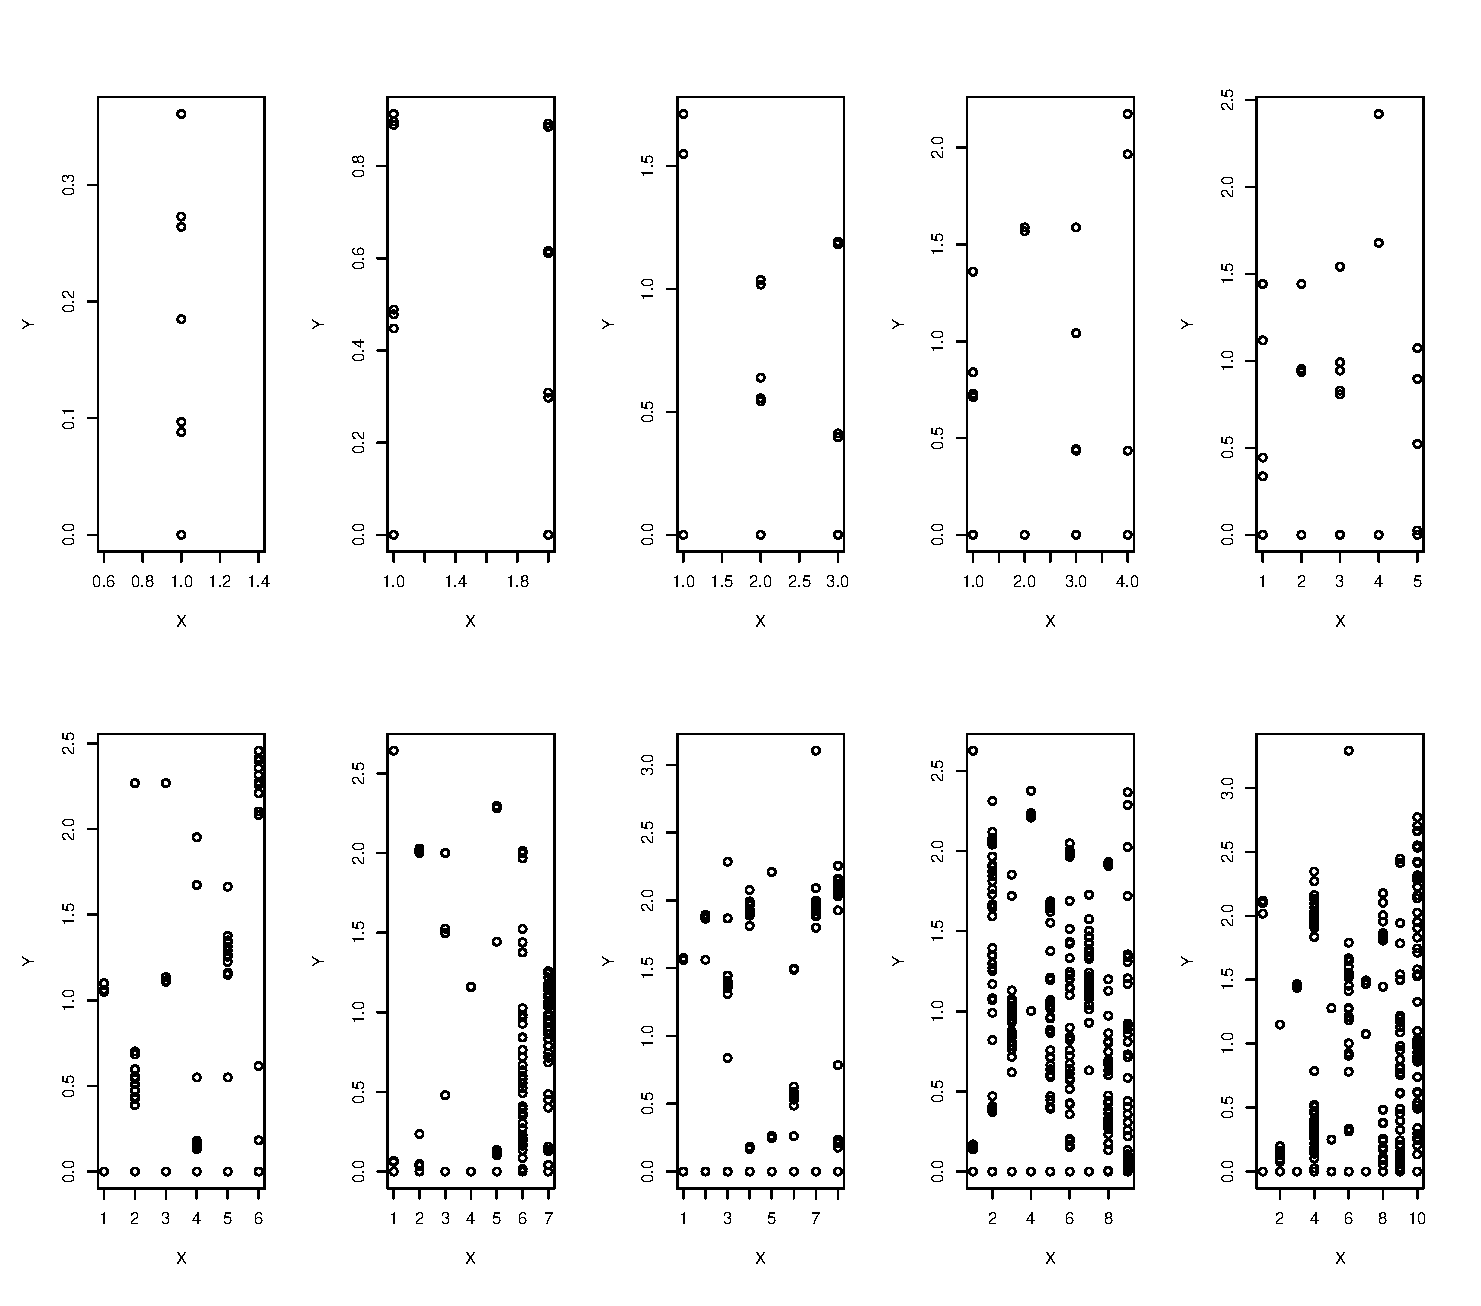
\includegraphics[width = 15cm]{pics/hw2_nmf_d_basis.eps}
\caption{NMF, D, basis, n=1:10}
\label{NMF_D1}
\end{figure}
And the error rate is as follows:
\begin{figure}[H]
\centering
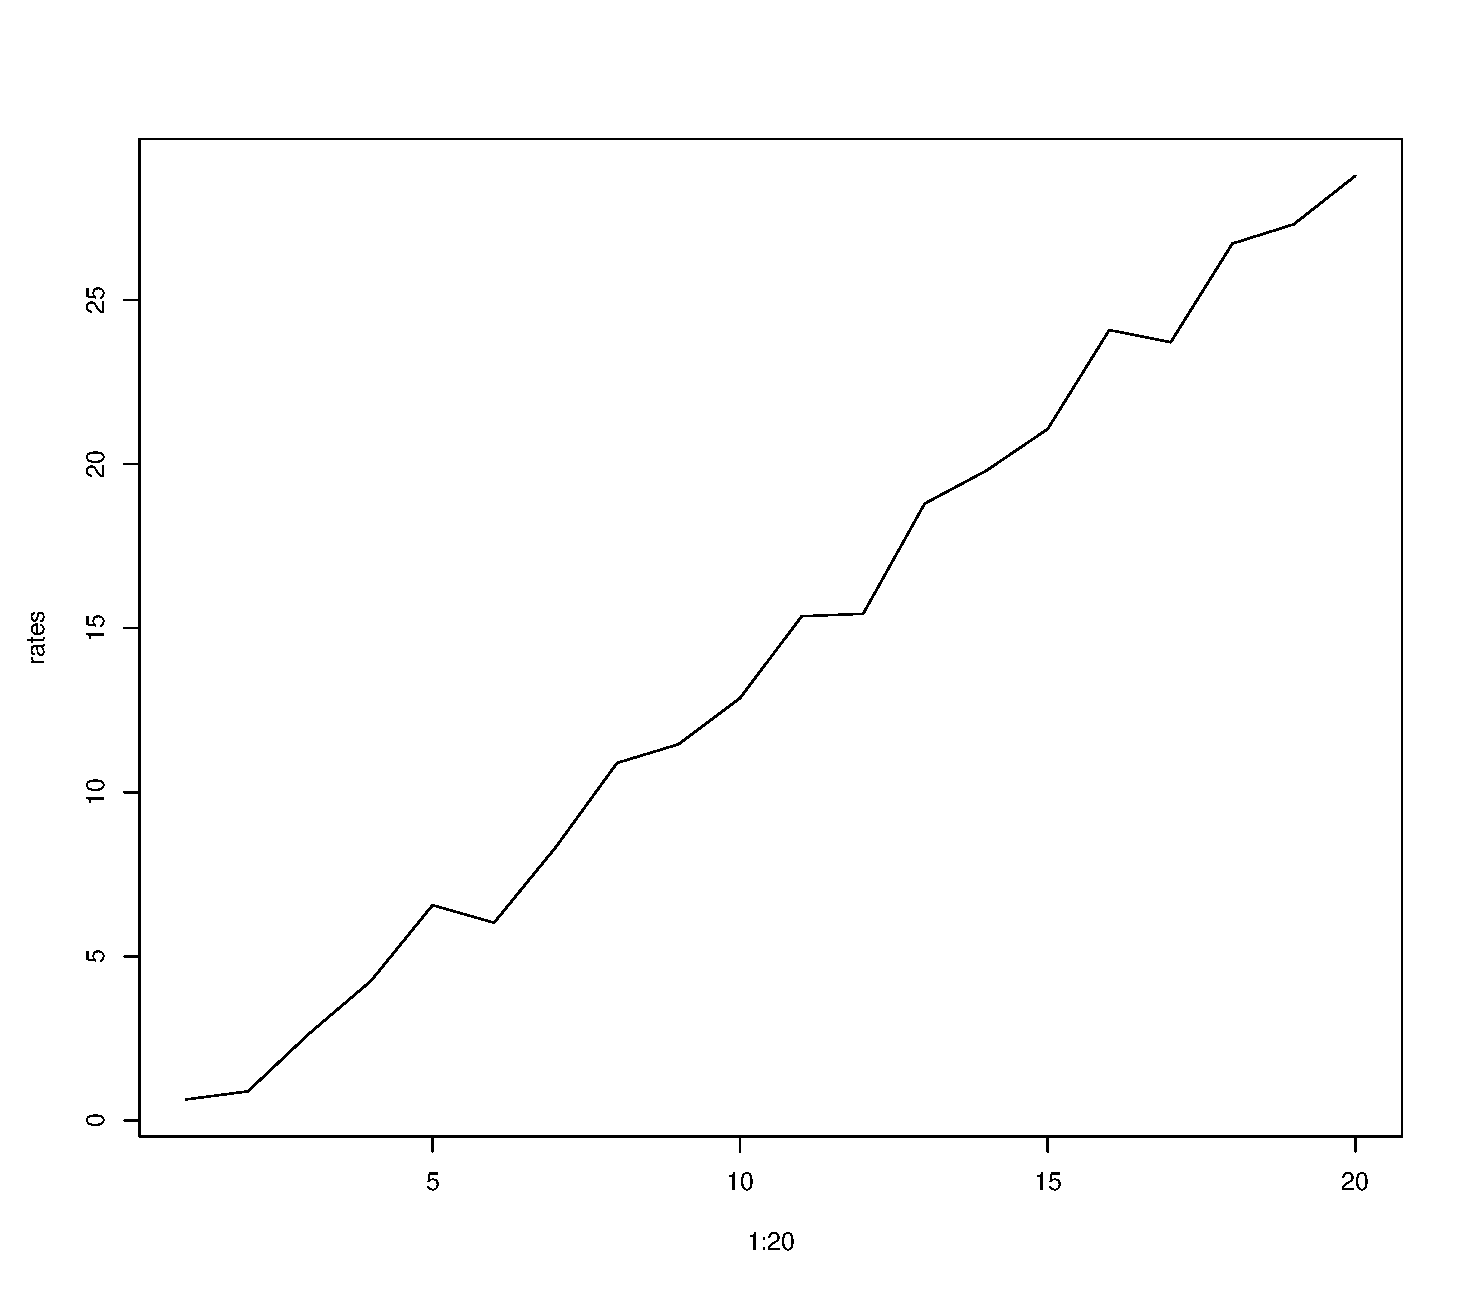
\includegraphics[width = 5cm]{pics/hw2_nmf_d_error.eps}
\caption{NMF, error rate, n=1:20}
\label{NMF_D2}
\end{figure}
From the curve of error rates we can know, that in this case the assumption that entries obeys Poisson distribution is not acceptable. So I tried Mean squared error objective function instead. In the meantime, MSE converged much quicker than D.\n
When using Mean squared error objective function
$$min\quad \vt{A-WH}_F^2$$
The basis is as follows:
\begin{figure}[H]
\centering
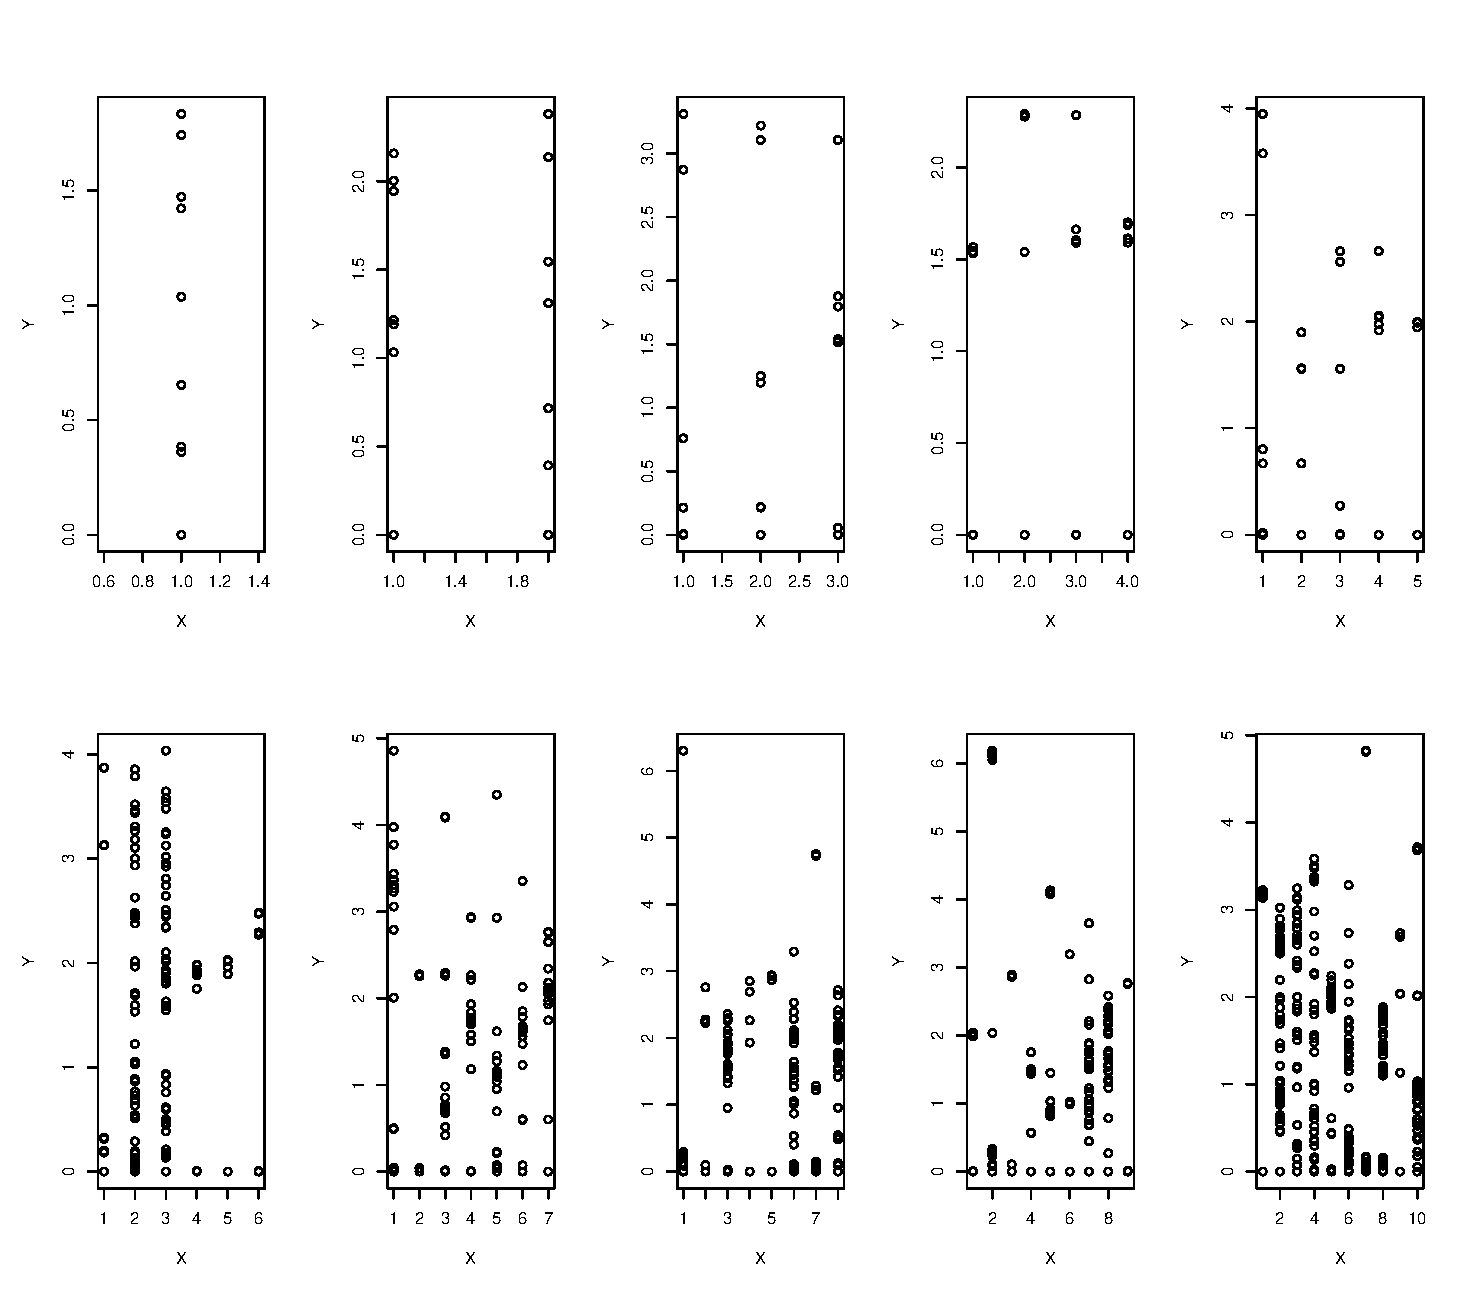
\includegraphics[width = 15cm]{pics/hw2_nmf_m_basis.eps}
\caption{NMF, M, basis, n=1:10}
\label{NMF_M1}
\end{figure}
And the error rate is as follows:
\begin{figure}[H]
\centering
\includegraphics[width = 5cm]{pics/hw2_nmf_m_error.eps}
\caption{NMF, M, basis, n=1:20}
\label{NMF_M2}
\end{figure}
One can tell from the error curve, that when we choose $k=6$, the result is good enough to represent the data from A.
}

\problem{3}{Perform PCA and NMF to test2.csv}
\solution{Analysis}{
When we do PCA to an image, we assume each row being a data point. Then PCA can be presented as
$$Y = XP$$
where $P$ is the matrix constructed by eigenvectors of $X\tr X$. Then 
$$X\tr X = P\Sigma P\tr$$
where $\Sigma$ is a diagonal matrix.
So choosing the first $k$ principle conponents is equivalent to choosing the first $k$ columns of $P$. We denote it as $P_1$.\n
If we let $A = XP_1 P_1\tr$, then
$$A\tr A = P_1 P_1\tr X\tr XP_1 P_1\tr = P_1 P_1\tr PDP\tr P_1 P_1\tr$$ 
$$ = P_1 D_{1:k} P_1\tr $$
So 
$$\hat{X} = XP_1 P_1\tr$$ is a approximation of $X$, and it is equivalent to restoring $X$ with its first $k$ singular values.
}
\solution{Result}{
For PCA, the result is shown as follows:\n
(I used Python-OpenCV to draw these images.)
\begin{figure}[H]
\centering
\includegraphics[width = 5cm]{pics/hw3_original.png}
\caption{Original Picture}
\label{Original}
\end{figure}
\begin{figure}[H]
\centering
\subfloat[k = 1]{ %
	\includegraphics[width = 0.3\textwidth]{pics/hw3_pca_1.png}}\hfill
\subfloat[k = 2]{
	\includegraphics[width = 0.3\textwidth]{pics/hw3_pca_2.png}}\hfill
\subfloat[k = 3]{
	\includegraphics[width = 0.3\textwidth]{pics/hw3_pca_3.png}}	
\end{figure}
\begin{figure}[H]
\centering
\subfloat[k = 4]{ %
	\includegraphics[width = 0.3\textwidth]{pics/hw4_pca_4.png}}\hfill
\subfloat[k = 5]{
	\includegraphics[width = 0.3\textwidth]{pics/hw3_pca_5.png}}\hfill
\subfloat[k = 10]{
	\includegraphics[width = 0.3\textwidth]{pics/hw3_pca_10.png}}	
\end{figure}
\begin{figure}[H]
\centering
\subfloat[k = 20]{ %
	\includegraphics[width = 0.3\textwidth]{pics/hw3_pca_20.png}}\hfill
\subfloat[k = 50]{
	\includegraphics[width = 0.3\textwidth]{pics/hw3_pca_50.png}}\hfill
\subfloat[k = 200]{
	\includegraphics[width = 0.3\textwidth]{pics/hw3_pca_200.png}}	
\end{figure}
For NMF, when we use Mean squared error obj func, the results are as follows:
\begin{figure}[H]
\centering
\includegraphics[width = 15cm]{pics/hw3_nmf_m.eps}
\caption{NMF, using MSE}
\label{hw3_NMF1}
\end{figure}
When we use Divergence squared error obj func, the results are as follows:
\begin{figure}[H]
\centering
\includegraphics[width = 15cm]{pics/hw3_nmf_d.eps}
\caption{NMF, using Divergence}
\label{hw3_NMF2}
\end{figure}
One can tell from the images that using mean squared error is almost the same as using divergence obj func, and their results are better than using PCA. I think it is because entries in a image are nonnegative, so if we use NMF, then the new basis are nonnegative which could be more appropriate.
However, since PCA can be performed easily using SVD, the speed of PCA is hundreds faster than NMF.
}
\end{document}